## Model system
The ASTAF-PRO system [@Kloas2015] was chosen as a model system for the estimation of aquafeed, alkalinity supplement, and source water mass flows into an exemplary aquaponic system. The sizing of the chosen system is comparable with results from a recent survey targeting aquaponics production sites [@Pattillo2022] and its system components are well-described. All model data are summarized in table \ref{tab:assumptions}.

```{=tex}
\begin{table}
\centering
  \caption{Rearing assumptions for the derivation of mass flows in aquaculture and aquaponic systems. Data originating from Kloas et al. (2015) with following additional assumptions: Stocking density represents the arithmetic mean of the minimum and maximum values reported. Average biomass was calculated from stocking density and rearing volume. Total water exchange rate reported was chosen instead of the supplied tap water.}
  \label{tab:assumptions}
  \begin{tabularx}{\textwidth}{XXX}
  \toprule
  Parameter & Unit &  Value \\
  \midrule

  Rearing volume & \si{\cubicm} & \num{7.91}\\
  Total volume & \si{\cubicm} & \num{13.0}\\
  Stocking density & \si{\kg\per\cubicm} & \num{48.8} \\
  Feeding rate & \si{\p\per\d} & \num{1.25} \\
  Water exchange rate & \si{\p\per\d} & \num{3.83} \\

  \addlinespace
  \hline
  \addlinespace

  Biomass & \si{\kg} & \num{386.0} \\
  Total feed input & \si{\kg\per\d} & \num{4.825} \\
  Total water input & \si{\cubicm\per\d} & \num{0.4979} \\

  \bottomrule
  \end{tabularx}
\end{table}

```



## Data collection and calculations

### Source water

```{=tex}
\begin{figure}
\centering
  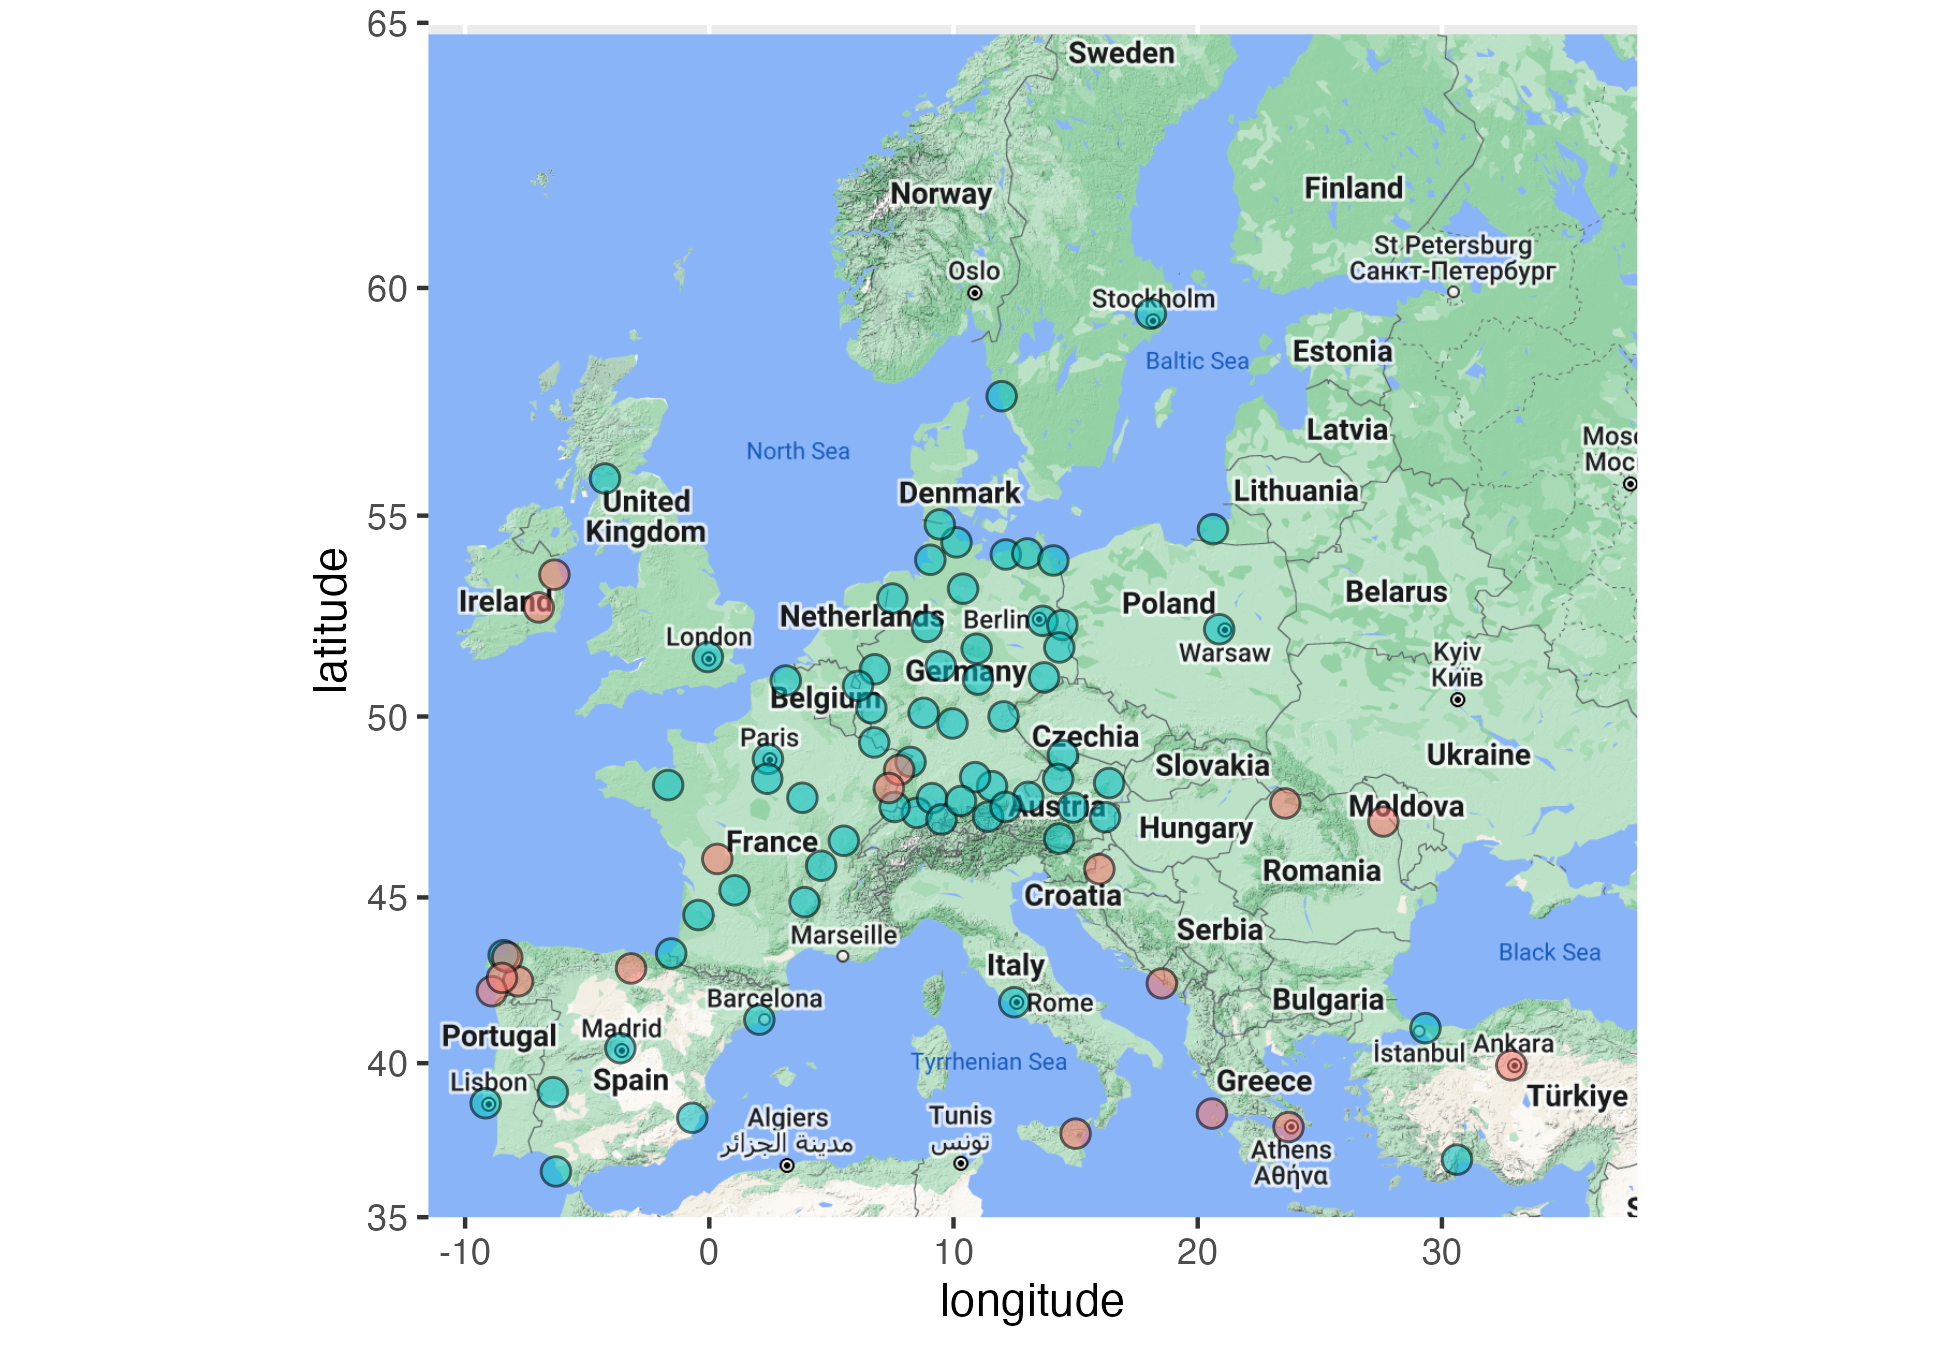
\includegraphics{../output/plots/map.png}
  \caption{Geographical distribution of water analysis reports included in the source water dataset. Green: analysis of municipal tap water; Red: rainwater analysis.}
  \label{fig:map_water}
\end{figure}
```

The total daily volume of freshwater introduced into the system (`r totalV * ER` \si{\L\per\d}) was calculated based on the model system. Daily plant nutrient inputs via source water were calculated by gathering tap water analysis reports from locations all over Europe. Official reports provided by local authorities and water utilities in the corresponding municipalities were used to ensure that analyses were conducted according to accepted laboratory standards. The collected `r results$n_wateranalysis` water analysis reports originated from a total of `r results$n_wateranalysis_countries` countries. 
Rain water analysis reports were collected from literature.
Their spatial distribution is shown in Figure \ref{fig:map_water}. 



### Aquafeeds
The total daily feed input $m_{in,total}$ (`r rearingV * SD * (FR/100)` \si{\kg\per\d}) was calculated based on the model system. Eventually, daily nutrient inputs via aquafeeds were calculated by multiplying the total daily feed input with the inclusion rates of the corresponding nutrient $\gamma_{X}$. As the study focusses on plant nutrients in aquaponic systems, nutrient retention by the livestock was considered, because it renders nutrients inaccessible for plants. This was done by multiplication of the total daily nutrient input with an \gls{adc} for each nutrient, yielding the true daily plant nutrient input via aquafeed. It was assumed that \gls{cp} digestibility would be on average \SI{90}{\p}, while the \gls{adc} for all other plant nutrients were assumed to be \SI{50}{\p} [@Lall2003]. Finally, due to the fact that solid substances are not accessible for plant uptake, it was assumed that \SI{50}{\p} of the digestible fraction is retained while the remaining \SI{50}{\p} is excreted in dissolved form [@Halver2003]. The calculation is described by equation \ref{eq:feed_input}.

```{=tex}
\begin{equation}
  m_{in,true} = m_{in,total} \cdot r_{feed} \cdot \gamma_{X} \cdot \text{ADC}_{X} \cdot r_{ex,diss}
  \label{eq:feed_input}
\end{equation}
```



### Alkalinity supplements
The input of alkalinity supplements was estimated based on @Timmons2010, with an amount of \SI{250}{\g} sodium bicarbonate (\ce{NaHCO3}) being recommended per \si{\kg} of feed input. Given the molar mass of \ce{NaHCO3} of $M(\ce{NaHCO3}) = \SI{84.01}{\gmol}$, this would translate into $n = \frac{m}{M} = \frac{\SI{250}{\g}}{\SI{84.01}{\gmol}} = \SI{2.975}{\mol}$ of \ce{HCO3-}, because $n(\ce{HCO3-}) = n(\ce{NaHCO3})$.  




## Data presentation, statistics, and software
All mass concentrations were converted to molar concentrations.

For statistical testing, a significance level of $\alpha = 0.05$ was chosen, unless otherwise stated.

In water analysis, it is common practice to report the value of the instrument detection limit instead of the measured value in case that the analyte concentration found was below the sensitivity of the measurement instrument [@ISO11843]. This practice is known as data censoring and used to ensure that the analyte signal can be distinguished from the instruments signal noise with satisfying confidence. However, retaining these data points in the dataset leads to incorrect results as the true concentration is within the interval from zero to the detection limit. To avoid an overestimation of plant nutrient concentrations within the tap water, true means from censored data were estimated by \gls{mle}, using the \emph{cenmle()} function from the R package NADA [@Helsel2011]. The calculated estimates were reported along with their \SI{95}{\p} confidence intervals.

All calculations were conducted using R (v4.2.2).
